\section{Problem Statement and Dataset Description}
\label{sec:problem_statement}

\subsection{Deep Learning Problem Formulation}
\label{sec:dl_problem}
We formalize chess as an autoregressive sequence modeling task over a discrete move alphabet, departing from conventional evaluation-search engines (e.g., minimax $\alpha$-$\beta$ pruning or MCTS). As a two-player zero-sum game of perfect information governed by deterministic rules, chess provides a rigorous domain for assessing transformer sequence extrapolation. A match $G$ of length $T$ plies is expressed as an ordered token sequence:
\begin{equation}
    \mathbf{x} = \left( x_1, x_2, \dots, x_T \right), \quad x_t \in \mathcal{V}
\end{equation}
where $\mathcal{V}$ is a finite vocabulary. The neural network parameterized by $\theta$ learns the joint probability distribution $P_\theta(\mathbf{x})$ factorized causally via the chain rule:
\begin{equation}
    P_\theta(\mathbf{x}) = \prod_{t=1}^T P_\theta(x_t \mid x_{<t})
\end{equation}
Parameters $\theta$ are optimized by minimizing expected cross-entropy loss over corpus $\mathcal{D}$:
\begin{equation}
    \mathcal{L}_{\text{CE}}(\theta) = - \mathbb{E}_{\mathbf{x} \sim \mathcal{D}} \left[ \frac{1}{T} \sum_{t=1}^T \log P_\theta(x_t \mid x_{<t}) \right]
\end{equation}
Figure~\ref{fig:ml_problem} illustrates this autoregressive framework, where the model attends strictly to historical move tokens ($x_{<t}$) to predict subsequent moves.

\begin{figure}[H]
  \centering
  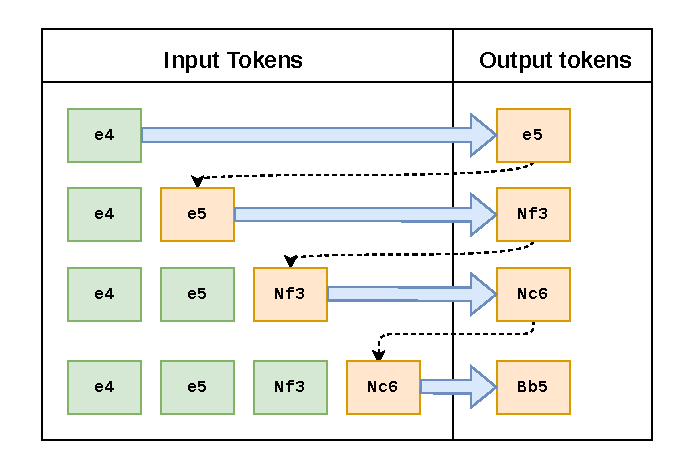
\includegraphics[width=0.82\linewidth]{figures/next_move_modelling.pdf}
  \caption[Autoregressive Next-Move Modeling]{Autoregressive sequence modeling framework for next-move prediction.}
  \label{fig:ml_problem}
\end{figure}

This formulation introduces three core representation challenges:
\begin{enumerate}
    \item \textbf{Absence of Spatial Inductive Bias}: The transformer receives no architectural priors regarding 2D grid topology, piece trajectories, or special constraints (castling, en passant, promotion).
    \item \textbf{Latent State Maintenance}: Because moves denote coordinate displacements rather than full board tensors, the network must internally track piece positions and pins over extended horizons.
    \item \textbf{Severe Action Sparsity}: At ply $t$, legal actions $\mathcal{A}_{\text{legal}}(s_t) \subset \mathcal{V}$ comprise an average of only 30--40 moves out of thousands of vocabulary permutations, leaving unconstrained sampling vulnerable to illegality.
\end{enumerate}

\subsection{Dataset Characterization and Acquisition}
\label{sec:dataset_char}
To train Nebium without overfitting to degenerate play, this project employs the \textbf{Lichess Open Database} \parencite{stockl-2021-watching}, which archives monthly competitive games in Portable Game Notation (PGN) format. We isolated an archival subset from January--February 2013 encompassing 245,293 tournament matches (Figure~\ref{fig:pgn_format}).

\begin{figure}[H]
  \centering
  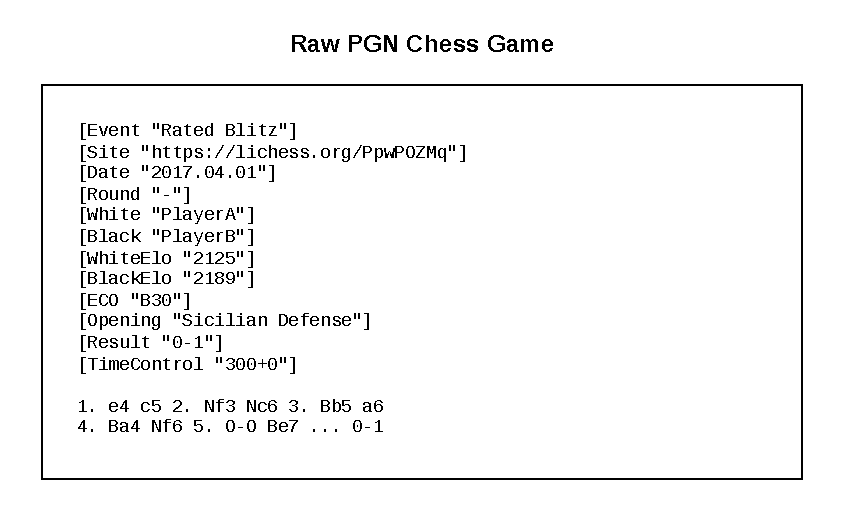
\includegraphics[width=0.78\linewidth]{figures/pgn_raw2.pdf}
  \caption[Representative Raw PGN Record]{Representative raw PGN record containing game metadata headers, standard algebraic notation (SAN), evaluation comments, and final match result.}
  \label{fig:pgn_format}
\end{figure}

\subsubsection{Data Filtering and Cleaning Pipeline}
Raw PGN dumps exhibit substantial variance in player expertise, clock aborts, and non-standard variants. An automated extraction pipeline (\texttt{src/data/prepare.py}) enforced four filtration criteria:
\begin{itemize}
    \item \textbf{Variant Filtering}: Retained standard chess games (\texttt{Variant "Standard"}), stripping chess960 and non-standard variants.
    \item \textbf{Game Length}: Discarded matches terminating in $<10$ plies; games exceeding 256 plies were truncated to the context limit.
    \item \textbf{Skill Floor}: Retained games where both players maintained an Elo rating $\ge 1500$, removing low-rated noise.
    \item \textbf{Metadata Stripping}: Discarded non-sequential metadata tags, isolating pure move strings terminated by match outcomes (\texttt{1-0}, \texttt{0-1}, \texttt{1/2-1/2}).
\end{itemize}
The filtered corpus comprises 208,412 games partitioned into \textbf{training} (85\%, 177,150 games), \textbf{validation} (10\%, 20,841 games), and \textbf{held-out test} sets (5\%, 10,421 games).

\subsection{Move Representation and Tokenization Strategy}
\label{sec:move_rep}
Standard Algebraic Notation (SAN)---such as \texttt{Nxf7+}---is human-readable but introduces linguistic ambiguity (e.g., disambiguation prefixes like \texttt{Nbd7}). To eliminate ambiguity, Nebium standardizes games into the \textbf{Universal Chess Interface (UCI)} coordinate format, where each move specifies Cartesian origin and destination squares:
\begin{equation}
    \label{eq:uci_format}
    m = \langle \text{file}_1, \text{rank}_1, \text{file}_2, \text{rank}_2, [\text{promotion}] \rangle \in \{\texttt{a1}\dots\texttt{h8}\} \times \{\texttt{a1}\dots\texttt{h8}\} \times \{\epsilon, \texttt{q}, \texttt{r}, \texttt{b}, \texttt{n}\}
\end{equation}
For example, moving a pawn from e2 to e4 is uniquely encoded as \texttt{e2e4}, kingside castling as \texttt{e1g1}, and queen promotion as \texttt{e7e8q}.

\subsubsection{Byte-Pair Encoding (BPE) Tokenization}
Tokenization critically governs transformer efficiency. Character-level tokenization expands sequence lengths by $4\times$, diluting attention across plies \parencite{stockl-2021-watching}. Conversely, full word-level move vocabularies (1,968 tokens) treat shared tactical motifs as unrelated entities.This project implements a custom BPE tokenizer via HuggingFace \texttt{tokenizers} (\texttt{ChessTokenizerHF}, Figure~\ref{fig:tokenizer}). Starting from ASCII characters, BPE iteratively merges co-occurring pairs up to $V = 5,000$ tokens, reserving control tokens:
\begin{equation}
    \mathcal{V}_{\text{special}} = \left\{ [\texttt{PAD}], [\texttt{UNK}], [\texttt{BOS}], [\texttt{EOS}], [\texttt{SEP}] \right\}
\end{equation}
Preserving whitespace boundaries enables the tokenizer to encode frequent opening lines and tactical exchanges (e.g., \texttt{e2e4 e7e5}) as single compound subwords, substantially compressing sequence length.

\begin{figure}[H]
  \centering
  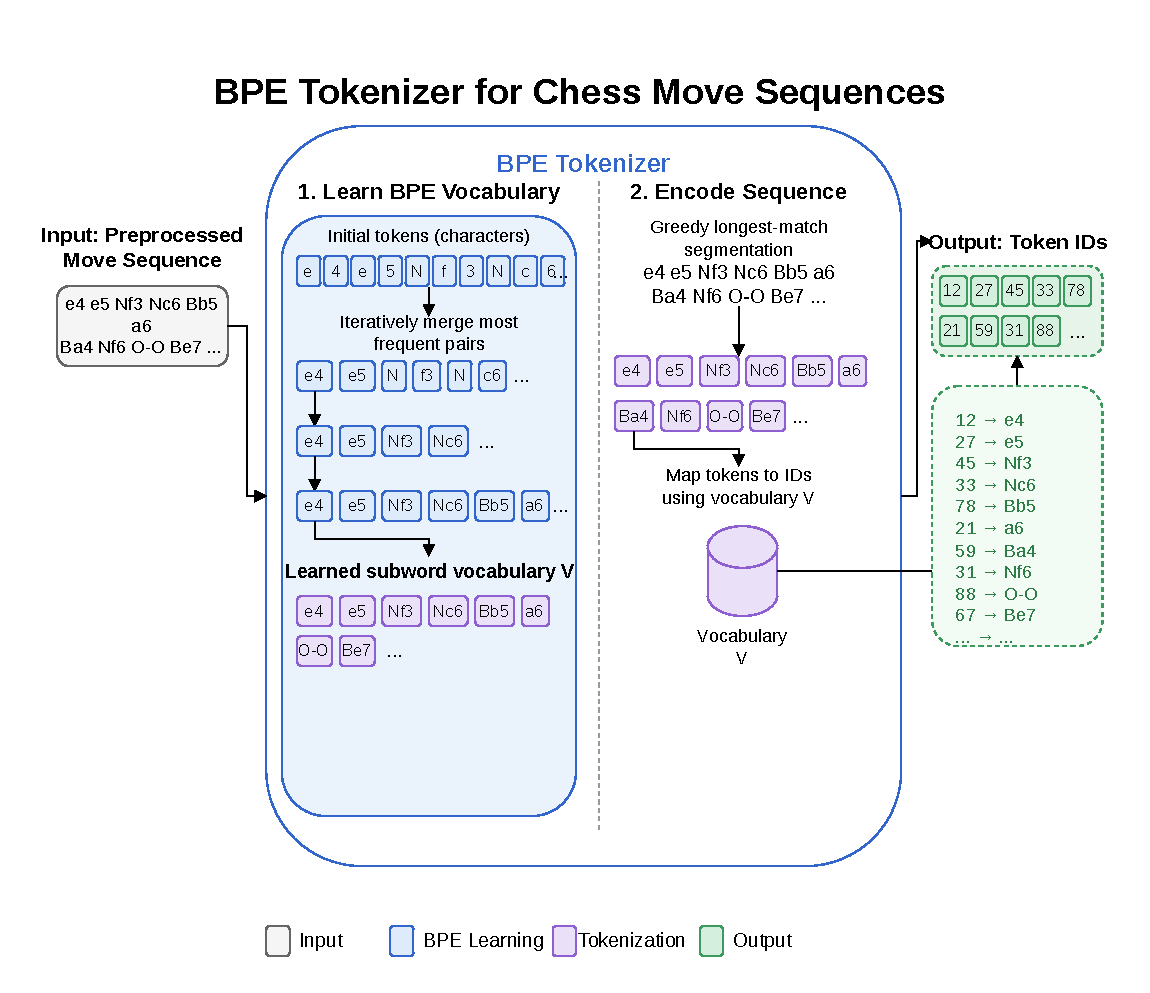
\includegraphics[width=0.88\linewidth]{figures/tokenizerChessBPE.pdf}
  \caption[BPE Tokenization Workflow]{Custom Byte-Pair Encoding (BPE) tokenization workflow implemented in \texttt{ChessTokenizerHF}.}
  \label{fig:tokenizer}
\end{figure}
